% Based on OSDI template:
% https://www.usenix.org/sites/default/files/osdi_submit.tex_.txt

% comment out the following line to move from EuroSec template to OSDI template
\newcommand{\isworkshoppaper}{X}

\ifdefined\isworkshoppaper
\newcommand{\paperdocumentclass}{sig-alternate-05-2015}
\else
\newcommand{\paperdocumentclass}{article}
\fi

\documentclass[10pt,twocolumn]{\paperdocumentclass}

% template packages
\ifdefined\isworkshoppaper
\else
\usepackage{times}
\usepackage{fullpage}
\fi

% non-template packages
\usepackage[bookmarks=true,pagebackref=false,pdftex]{hyperref}
\usepackage{epsfig} % eps figures
\usepackage{graphicx}
\usepackage{epstopdf}
\usepackage{cite}
\usepackage{verbatim}
\usepackage{listings}
\usepackage{xcolor}

% variables
\newcommand{\projectname}[0]{METAlloc}

% comment out the following line to disable comments in text
%\newcommand{\commentsenabled}{X}
% comment commands
\ifdefined\commentsenabled
\newcommand{\EK}[1]{\textbf{\color[rgb]{0,1,0} EK: #1}}
\newcommand{\IH}[1]{\textbf{\color[rgb]{1,0,0} IH: #1}}
\newcommand{\CRI}[1]{\textbf{\color[rgb]{0,0,1} CRI: #1}}
\else
\newcommand{\EK}[1]{}
\newcommand{\IH}[1]{}
\newcommand{\CRI}[1]{}
\fi
\newcommand{\lipsum}[1]{{\color[rgb]{0.75,0.75,0.75} Lorem ipsum dolor sit amet, consectetur adipiscing elit, sed do eiusmod tempor incididunt ut labore et dolore magna aliqua. Ut enim ad minim veniam, quis nostrud exercitation ullamco laboris nisi ut aliquip ex ea commodo consequat. Duis aute irure dolor in reprehenderit in voluptate velit esse cillum dolore eu fugiat nulla pariatur. Excepteur sint occaecat cupidatat non proident, sunt in culpa qui officia deserunt mollit anim id est laborum.}}



\lstset{language=C++, 
    frame=lines, 
    backgroundcolor=\color{white},
    basicstyle=\scriptsize,
    %numbers=left,
    breaklines=true,
    tabsize=2,
    captionpos=b,
    commentstyle=\color{gray}\ttfamily,
    xleftmargin = 6pt,
}

\hypersetup{
unicode,
% no color links
colorlinks=true,
citecolor=black,
filecolor=black,
linkcolor=black,
urlcolor=black
} 

% hacks
\newenvironment{code}{\small\verbatim}{\endverbatim\normalsize}
\newcommand{\note}[1]{\noindent\textbf{\color{red}[#1]}}
\newcommand{\commentout}[1]{}

\begin{document}

\ifdefined\isworkshoppaper
\title{\projectname{}: Efficient and Comprehensive Metadata Management for Software Security Hardening}
\else
\title{\bf \projectname{}: title goes here} % TODO put title here
\fi

\ifdefined\isworkshoppaper
\author{
	Istvan Haller \\ Vrije Universiteit Amsterdam \\ \texttt{i.haller@student.vu.nl} \and 
	Erik van der Kouwe \\ Vrije Universiteit Amsterdam \\ \texttt{vdkouwe@cs.vu.nl} \and 
	Cristiano Giuffrida \\ Vrije Universiteit Amsterdam \\ \texttt{giuffrida@cs.vu.nl} \and 
	Herbert Bos \\ Vrije Universiteit Amsterdam \\ \texttt{herbertb@cs.vu.nl}}
\else
\author{Paper \# XXX} % TODO put paper number here, no author names as submission is double-blind
\fi

\date{}
\maketitle
\thispagestyle{empty}

\begin{abstract}
% What is the problem?
Many system applications are still developed using unsafe languages like C/C++. Memory corruption due to dangling pointers in these applications can lead to Use-after-Free (Double-Free) vulnerabilities. Many Use-after-Free detection schemes and systems have been proposed in the previous work. These systems either incur high performance overhead or have limited applicability.
% What we did?
This paper proposes \projectname{}, a simple and efficient lock-less system to prevent Use-after-Free exploits during runtime. \projectname{} uses LLVM compiler instrumentation pass to insert run-time pointer tracking functions. During run-time, most of the pointers that point to the object are tracked. These pointer values are set to invalid addresses when the object is freed. \projectname{} is based on efficient metadata management framework, \metalloc{}~\cite{istvan2016metalloc}.
% How we did?
% what we achieved
 It has moderate performance overhead. For SPEC2006 benchmarks, it has $43.9\%$ average (geometric mean) run-time overhead when only heap pointers are tracked. For widely used web-servers (\texttt{nginx}, \texttt{httpd} and \texttt{lighttpd}), it has moderate throughput degradation of $12.8\%$ and negligible service latency overhead. Moreover, \projectname{} successfully prevented recently discovered Use-after-Free vulnerabilities in widely used complex software.
\end{abstract}

\section{Introduction}
\label{sec:introduction}

Many common software security hardening solutions need to maintain and look up
memory metadata at runtime. Examples include bounds information to validate
array references~\cite{akritidis2008preventing,akritidis2009baggy}, type information to validate cast operations~\cite{lee2015type}, solutions that prevent use-after-free exploits~\cite{lee2015preventing,younan2015freesentry},
and object pointer information to perform garbage collection~\cite{rafkind2009precise}.
While newer programming languages can often track
such metadata in-band using fat pointers, previous efforts to implement
in-band metadata management in systems programming languages, such as C or C++,
have found limited applicability due to poor ABI compatibility and nontrivial overhead~\cite{dhurjati2006backwards}.

The alternative solution is to associate metadata information with the memory objects themselves, assuming we have a mechanism to map pointers to the appropriate metadata.
Such a  primitive is the key to implementing  modern metadata management schemes,
%% given 
but it is also challenging because it needs to support all the possible memory objects (heap objects allocated
with \texttt{malloc()}, globals, and stack objects)
as well as minimize the performance and memory impact
of metadata update and lookup operations.

Minimizing the impact of update operations
is challenging,
because allocation and deallocation of memory objects and their metadata occurs frequently during execution. 
%% many memory objects (e.g., stack objects) and their metadata are
%% frequently allocated/deallocated during the execution.
Minimizing the impact of lookups is also
challenging, since metadata lookup must be able to support interior pointers
into nested classes, structures, and arrays---dictating support for range queries and disqualifying the use of space- and time-efficient hash tables.
\looseness=-1

Current state-of-the-art software hardening projects all rely on tailored, mostly one-off 
solutions for metadata
management, but none of them simultaneously achieves low lookup and update impact in all cases. As a result, none
of them provides a generic solution. 
Common approaches include tree-based metadata handling and memory shadowing.
 
Tree-based approaches~\cite{haller2013mempick,lee2015preventing} store
an interval node for each allocated object according to to its bounds.
Unfortunately, tree lookups can result in a prohibitive performance hit,
as the tree depth is frequently in the double digit range (more than 1,024 memory objects).
The lookup time is also unpredictable, as it varies with the object count.
As a result,  tree-based systems are unsuitable
for most production situations.
\looseness=-1

Traditional memory shadowing, in turn, relies on a fixed
pointer-to-metadata mapping~\cite{akritidis2008preventing,akritidis2009baggy,younan2015freesentry},
The key design choice for this approach is the \emph{metadata compression ratio}.
The metadata compression ratio represents the number of metadata bytes that need to
be tracked for each data byte.
For example, assume we store one byte of metadata for each block of eight bytes.
In this case the compression ratio is $\frac{1}{8}$. If we have a pointer $p$ and
an array of metadata starting at address $q$, we can compute a pointer
to the metadata for object as $\frac{1}{8} p + q$.
This way, metadata can be located very efficiently.
However, choosing the appropriate
compression ratio is difficult, as it enforces a minimum alignment on every memory allocation.
Small compression ratios result in inflated metadata size and a large tracking overhead,
while large compression ratios result in significant memory fragmentation.
In practice, memory management systems typically only guarantee alignment
up to 8 or 16 bytes. This means that to keep the compression ratio reasonably
small only a single byte of metadata is supported~\cite{akritidis2008preventing,akritidis2009baggy}.
Even then, this approach introduces prohibitive initialization time and
memory overhead for large objects in case multi-byte metadata is needed.
Finally, recent approaches rely on custom
allocators to reduce the impact of memory shadowing on the heap, but
cannot support efficient and comprehensive metadata management
including more performance-sensitive objects on the stack~\cite{lee2015type}.

In this paper, we propose \projectname{}, a new metadata memory management scheme
based on an efficient and comprehensive variable memory shadowing strategy. Our
strategy builds on recent developments in heap~\cite{ghemawat2009tcmalloc} and stack~\cite{kuznetsov2014cpi} organizations
to implement a variable and uniform pointer-to-shadow mapping
and significantly reduce the performance and memory impact of metadata management.
Our results show that \projectname{} is practical and can support efficient
whole-memory metadata management for several software security hardening solutions.

Summarizing, we make the following contributions:

\begin{itemize}
%\setlength\itemsep{1.5em}
\item We propose a new memory metadata management scheme that supports interior pointers
      and is time- and space- efficient in both lookups and updates across all memory object types.

\item We present a prototype implementation termed \projectname{},
      which demonstrates that efficient and comprehensive metadata management is feasible and widely applicable in practice.

\item We present an empirical evaluation showing that \projectname{} incurs a run-time performance overhead of just 1.2\% on SPECint2006.
  
\end{itemize}

\section{\projectname{}}
\label{sec:metalloc}

As we have seen, one of the major limitations of state-of-the-art
memory shadowing approaches is the difficulty of getting the compression ratio right.
Because the right value may differ from application to application, the
intuitive solution is to enable a variable compression ratio.
This eliminates the fixed memory overhead associated with metadata shadowing
and greatly reduces the allocation-time performance hit.
%It also introduces the need for an additional mechanism to infer the appropriate compression ratio
%during metadata retrieval.
\begin{comment}
This scheme is used in the sanitizer library of LLVM as a means to track metadata
with manageable memory overhead. 
It groups most heap allocations into regions based on their size, with each region organizing objects
into buckets of a unique size. Intuitively each region is associated on the largest possible compression ratio,
mapping each bucket to one piece of metadata. Lee et al.~\cite{lee2015type} showcase it as
effective for checking the type safety of cast operations at run time, but they also 
highlight some limitations, such as the inability to use this metadata tracking system
for global and stack objects. The allocator also lacks address randomization and
the ability to reclaim physical memory, making it unsuitable
for general purpose deployment.
%\EK{we are no longer presenting this in this paper; should we bring it back?}
% For an arena-based system this
% is equivalent to identifying the arena which owns the pointer itself. This
% process has not yet been designed with performance in mind within the LLVM implementation.
\end{comment}

\projectname{}'s key goal is to implement a metadata management scheme
handling all memory objects in a uniform and highly efficient manner, regardless of
their allocation type (heap, stack, or global memory).
There are two requirements 
to accomplish this goal.
The first is to support a simple, efficient, and uniform mechanism
to associate pointers with the compression ratio. The second is the
ability to optimize the compression ratio as much as possible, ideally such that only a single
metadata entry is needed for each object. \projectname{} meets both these requirements
by ensuring that all the memory objects within a memory page
share a nontrivial common alignment, which is fixed
as long as there are active objects within the page. 
This requirement serves as a basis for our scheme and is met
by drawing from modern heap~\cite{ghemawat2009tcmalloc} and stack~\cite{kuznetsov2014cpi} organizations
widely used in production, as discussed in Section~\ref{sec:assumptions}.
\looseness=-1

Alignment relates directly to the compression ratio, namely an $n$-byte object
alignment allows one \emph{metadata entry} to be associated to every group of $n$ bytes
within said object. Having uniform alignment within each memory page allows 
\projectname{} to associate compression ratios to the individual memory
pages and to look them up using a mechanism similar to \emph{page tables}. Such page tables
also include the location of the metadata region corresponding to the individual pages.
This mechanism is described in the following section.

\subsection{Efficient retrieval of page information}
\label{sec:pageinfo}

Because lookups are expected to be very frequent, the page table design is very
performance-sensitive. For this reason, \projectname{} opts for a single-level page table design,
which requires only one memory read for each lookup. We refer to this data structure as the
\emph{meta-page table}. 
Figure~\ref{fig:metalloc} shows the general operating principle of \projectname{},
including the use of the meta-page table.
Given a pointer, we spit it in a page index and an offset.
The page index is used as an index into the meta-page table,
which is an array stored at the page table base.
This page table base is a compile-time constant and therefore requires no extra memory read.
The entries in this array are eight bytes large, split between the seven-byte \emph{metabase} pointer and
the one-byte base-2 logarithm of the memory alignment.
The metabase points to the start of an array of metadata entries
available for this page table entry.
The size of the entries of the metadata array is determined by the \emph{metasize}
compile-time constant, which specifies the amount of metadata per object.
It should be noted that objects larger than the alignment size have multiple
metadata entries, each with the same contents.
The offset part of the original pointer divided by the alignment serves
as an index into the metadata array, allowing the correct metadata entry to be
located for the specified object.

\begin{figure}[t]
\center
  \includegraphics[width=3.5in]{figs/metalloc.pdf}
  \caption{
  \projectname{}'s metadata lookup
  }
  \label{fig:metalloc}
  \vspace{-1em}
\end{figure}

While the size of the meta-page table (for x86-64 systems using 48-bit virtual addresses and 4096-byte pages)
is theoretically $2^{36}$ entries or $512$ GB, only pages corresponding to address ranges currently in use by the process need to be allocated. To implement this strategy, \projectname{} reserves the required virtual memory area in advance and relies on demand paging to lazily link the required page table pages to physical memory.
\begin{comment}
A backup mechanism
is necessary to stop the continuous expansion of the meta-page table as the program potentially
migrates its data from one virtual address range to another during execution (for address randomization for instance).
\end{comment}
\looseness=-1

\begin{comment}
We solve this problem by including a secondary ref-count table which tracks the usage of the meta-page table.
Whenever we detect that a virtual page within the meta-page table becomes unused by the process, we notify the
OS to release the underlying physical storage. The ref-count table only needs a two-byte counter for 
each virtual page of the meta-page table, limiting its size to
$2^{27}$ entries or $256$ MB of virtual memory. This can be further reduced
by grouping multiple pages in the same entry. The ref-count table is accessed and manipulated only during \texttt{mmap}
and \texttt{munmap} operations (when the virtual address range of the process changes),
thus it does not affect the critical path of the program.
\IH{don't we jut take out the hit-count table for EuroSec and mention it briefly?}
\end{comment}

\subsection{Static versus dynamic metadata}
\label{sec:metadata}

The scheme presented so far assumes a fixed-sized metadata entry
which is statically initialized at the start of the object's lifetime.
For objects whose size exceeds their alignment there are multiple copies
of this metadata entry in memory.
A metadata entry can be an integer, a small struct
or even a pointer, which can refer to further metadata of arbitrary dynamic size.

\CRI{We always talk about amount of metadata to refer to both ``sizeof(user-metadata)'' and ``sizeof(user-metadata)*copies''. We need make a clear distinction between the two in the paper, or readers will be lost. For instance, the term ``metadata node'' appears out of the blue below, while it should appear much earlier.}\EK{we now consistently use ``metadata entry'' for the metadatta array and ``metadata node'' just for the same-lifetime objects, IMO this fixes the ssue; I also added mentions of copies of the entries}
In the simplest possible setup, each metadata entry is filled with a compile-time constant,
such as a type index. This scheme allows the instrumentation to identify certain predetermined object characteristics at run time, with the lowest possible overhead. In this use case, initializing the
metadata is cheap, as it involves a simple \texttt{memset} operation for the compressed metadata range corresponding to the object. Given the use of variable compression rates, the amount of metadata that needs to be initialized is minimal.

Alternatively, the metadata can include a pointer to information created
at compile time in global memory. This scheme may be, for example, used to
support in-depth type tracking when implementing precise garbage collection
for languages such as C/C++~\cite{rafkind2009precise}.
From an overhead perspective, this is similar to the constant metadata scenario, as the pointer itself is just another numeric constant,
% (or a PC-relative value)
whose value is fixed at compile time.

Finally, the metadata pointer might be generated at run time.
In this case, a \emph{metadata node} is allocated whenever a new memory object
is allocated and deallocated when the memory object is. 
This scheme is relevant to instrumentation tailored to individual object
instances, rather than broad object groups. Sharing lifetimes is trivial on the
stack and in global memory, but leads to interesting design decisions when dealing
with the heap. Intuitively, the fastest solution is to increase the allocated size
of the object itself and store the metadata node in-band. In practice, we found
this solution to result in significant performance degradation due to its
negative caching impact.
The alternative is to perform a second heap allocation dedicated to the metadata node 
itself. While we expected a nontrivial performance hit for applications where allocations
dominate the run time, we found the impact to be reasonable in practice.
% We suspect that
% this is made possible by the efficiency of tcmalloc when allocating from a homogeneous
% pool of fixed-sized objects.
In addition, most applications do not require object-specific metadata tracking
and can safely refrain from using dynamic metadata, as it incurs the highest run-time and memory overhead.
\CRI{We don't discuss metadata integrity at all here. This may be fine for EuroSec if we don't have any story at all, but I suspect the solution to have both performance and integrity is to allocate the deep metadata node right after the first pointer copy (forcing a larger minimum alignment).}\IH{Not alignment per-se, but you force each metadata node to be significantly larger.}

\subsection{Instrumentation across memory types}
\label{sec:assumptions}

\textbf{Globals}. Global memory is the simplest to deal with from a memory shadowing perspective. Global allocations only occur at load time and the amount of global data is typically
limited. These properties suggest that the default 8-byte alignment within the system works reasonably well for this allocation type, thus we can just associate every global data memory page with this alignment in the meta-page table.
We simply instrument binary files (executables and dynamic libraries) to allocate metadata pages and set up the meta-page table entries corresponding to their data sections as soon as the binaries are loaded.

\textbf{Stack}. Stack pages share the property of long lifetimes with global memory (associated with the stack for the lifetime of the thread), but they are unique in that object allocations within the pages occur frequently and with minimal run-time cost. A simple solution is to restrict stack objects to the conservative 8-byte alignment~\cite{akritidis2008preventing},
% since the stack also includes a number of spilled registers or ABI specified elements
% which have restricted movement.
but this makes tracking multi-byte metadata
prohibitively expensive. \projectname{} solves this challenge by leveraging recent advances
in shadow stack solutions (recently integrated in mainstream compilers)~\cite{kuznetsov2014cpi}, which split the program stack into a primary and a secondary stack.
\projectname{} uses a multi-stack approach with a primary and a number of secondary stacks.
The primary stack preserves all the stack objects not subject to
the current instrumentation, including ABI specific elements such as
return addresses and arguments, while the secondary stacks store the remainder. The secondary stacks each are designed for a particular
class of object sizes with appropriate non-trivial alignment to improve the compression ratio for metadata tracking.
This design ensures that \projectname{} only needs to care about the secondary stacks, which are free from ABI specific restrictions.
We propose using the same heuristic for all instrumentations, namely moving all objects which can potentially be subject to memory
corruption attacks (either address taken or address used in unpredictable manner) to one of the secondary stacks. In practice the secondary stacks end up composed
mostly of arrays and some address taken integers. As a result, we propose enforcing a relatively
large alignment on each object within every secondary stacks. While some memory fragmentation
does occur with address taken integers, it only affects a small portion of the entire
memory address space of the program and it will not break program functionality in general.
Our current design uses one secondary stack for small and medium objects having a fixed alignment of 64 bytes,
and another secondary stack for large objects where 4096 byte alignment is enforced.
\projectname{} instruments the allocation of program stacks to create the secondary stacks
and to also allocate the corresponding metadata pages and to set up the appropriate meta-page table entries.

\CRI{As above, we need to make this design section self-contained and not using oblivious writing (i.e., we're like X except plus Y and minus Z). We can say we draw from recent allocator design (tcmallocREF) to organize the heap as X, Y, Z to match our assumptions (as above), but then we have to explain things end-to-end and forget about tcmalloc here. We can just have the next (short) subsection named Implementation, which mentions ``We implemented METAlloc in etc. etc. For stack management, we modified SafeStack to do X. For heap management, we modified tcmalloc to do Y.}
\textbf{Heap}.
In order to meet our requirements,\projectname{} uses a heap allocator designed around the concept of object sizes.
Instead of keeping track of the heap as a whole, it operates with size-specific free-lists instead.
Whenever a free-list becomes empty, the allocator can request new memory pages from the system, which are
then associated with this particular free-list until they are released back to the system. The allocator would then
enforce the largest possible alignment for objects within each free-list without triggering too much
fragmentation. Applying \projectname{} to such a heap allocator is trivial as one just needs to monitor
page request by the free-lists to associate the appropriate metadata information with the pages. Figure~\ref{fig:metalloc-heap}
summarizes this operation with the addition of potential object caches and a page allocator to improve performance.

\subsection{Implementation specifics}
\label{sec:assumptions}

While it is possible to build a new custom heap allocator which respects our design specification
, we decided to build upon a proven, state-of-the-art allocator instead. We expect that for most
complex C++ applications the heap allocator has a significant impact
on performance, thus a proven allocator is key. The tcmalloc allocator 
(developed and used by Google) features a memory organization which matches our requirements.
\looseness=-1

For the stack we decided to extend the implementation of SafeStack~\cite{kuznetsov2014cpi}, as it is advertised
as a replacement for stack canaries going forward and it is becoming a core component within the LLVM
project. Its interpretation of safe and unsafe objects also matches up well with our definition of objects
requiring instrumentation. 

\begin{comment}Its central free list operates on the basis of memory spans. Each span is a set of contiguous memory pages
configured to include a specific class of objects defined by their size. These spans
are allocated and deallocated monolithically, the central free list not having
control over the span configuration. The allocator ensures the same alignment 
(as large as possible, while restricting fragmentation) for all the objects 
within a span. We extend tcmalloc by allocating metadata pages and updating
the meta-page table whenever a new span is allocated. Figure~\ref{fig:metalloc-heap}
summarizes this operation.\end{comment}

\begin{figure}[t]
\center
  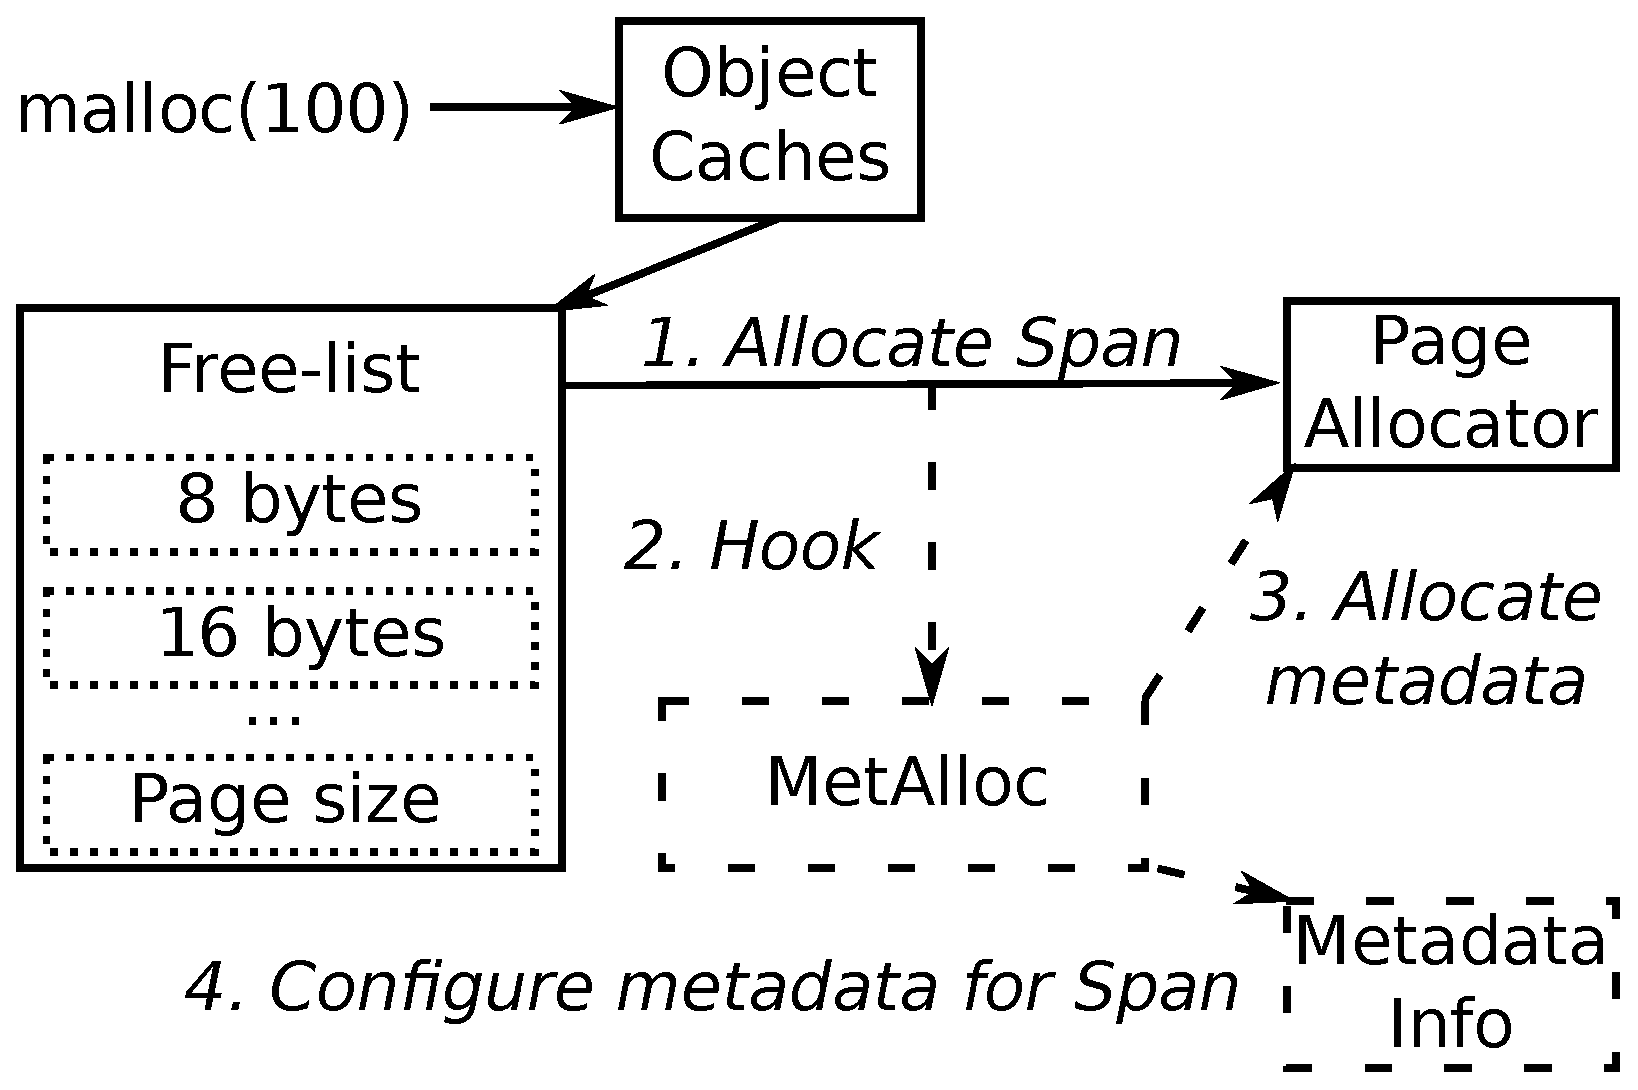
\includegraphics[width=2.8in]{figs/metalloc-heap.eps}
  \caption{
  Heap metadata management using \projectname{}
  }
  \label{fig:metalloc-heap}
  \vspace{-1em}
\end{figure}



\section{Applications}
\label{sec:applications}
\CRI{I suspect this section will have to go for EuroSec (and be condensed as a couple
of examples in the intro.)}

Efficient metadata tracking enables a wide range of valuable instrumentation
tools to be used with production systems where performance overhead is a
key characteristic. In the following we present a couple of key examples 
of such instrumentation.
% and their design relative to \projectname{}. 
This list is by no means exhaustive and we hope that readers
find other innovative uses of the framework. In this (short) paper, the applications  serve as motivation for our work and we will focus our evaluation on the framework itself.

\subsection{Write Integrity Protection}

Recent developments in attack techniques~\cite{carlini2015control,evans2015control,schuster2015counterfeit}
show the need to enforce additional data 
integrity within the program besides the classic control-flow integrity. 
Both Microsoft's WIT~\cite{akritidis2008preventing} and Oracle Application Data Integrity have looked into the 
topic of restricting the target addresses of memory writes using a coloring mechanism. 
In these schemes each memory location is associated with a given color and the instrumentation
alongside each memory write checks if the target location matches the color of
the pointer/instruction.
The major difference between the two schemes is the availability
of pointer color in the Oracle implementation stemming from a custom extension in
their latest CPU design. Microsoft on the other hand computes static colors for
the instruction based on points-to analysis.
In the case of both of these systems, the color for the memory location is tracked
using metadata shadowing with a fixed compression ratio.
Replacing these systems with \projectname{} can lead to substantial improvements  in  allocation performance.

In the case of both of these systems, the color for the memory location is tracked
using metadata shadowing with a fixed compression ratio. Thus integrating \projectname{}
into these systems is trivial, bringing with it all the advantages of variable compression ratio,
namely lower memory overhead and lower allocation overhead. However it does introduce
overhead when retrieving the metadata as the metadata information also needs to
be retrieved for the memory page corresponding to the pointer. In practice Write Integrity Protection
requires the most frequent metadata retrieval out of all the presented applications, showcasing the
worst case behaviour of \projectname{}.
\begin{comment}
To measure the effects of integrating \projectname{} into these systems, we
reimplemented the Microsoft scheme in a simplified manner. We use the DSA inter-procedural
points-to analysis~\cite{lattner2007making} from LLVM to identify connections between instructions
and memory locations. Since we only care about the performance characteristics of the metadata
tracking component, the accuracy of DSA relative to the points-to analysis presented in
the WIT paper is irrelevant. We also replicate the original metadata tracking from WIT by fixing the compression
ratio to the proposed values and by using a shadow memory located at a fixed address, allowing us to
perform a fair comparison across more recent benchmarks.
We also preserve the original design using a single byte of color as metadata. The detailed comparison of
the different metadata tracking solutions for write integrity protection can be found in
section~\ref{sec:evaluation}.
\end{comment}

\subsection{Bounds Checking}

Efficient bounds checking has been proposed in the past to counter
buffer overflow vulnerabilities, but none of the solutions ended up in production systems
due to the performance and memory overheads they bring. One particularly efficient example is
Baggy Bounds Checking~\cite{akritidis2009baggy} which offers a strong protection model with limited memory overhead,
based on fixed compression metadata. Its primary deficiency is the need to allocate objects in slots
with sizes in the powers of two, a requirement that is typically not enforced in generic heap allocators
due to the potential for high internal fragmentation.
The system can be rebuilt without the alignment requirements but that would require tracking
base pointer and size information for every object, which leads to performance and memory issues with
the fixed compression ratio (it is prohibitive to store 16 bytes of metadata for every 8 data bytes).
\projectname{} and its variable compression ratio can help to deal with the problematic large object allocations,
ensuring consistently low overhead across applications even when using multiple metadata bytes.

For this application the design requires a 16-byte metadata including both base pointer and size information.
Metadata retrieval is performed whenever a potentially dangerous pointer is read from memory and bounds check is applied to
pointer arithmetic with the same logic as defined in Baggy Bounds Checking. Again metadata retrieval is more expensive than with
the shadowing approach, however it occurs significantly less frequently. Most of the time pointer arithmetic suggests accesses to
multiple different offsets relative to the same base pointer, allowing the instrumentation to reuse the pointer metadata for multiple
bounds checks.
\begin{comment}
\EK{ISTM it's not really the same because the alignment in baggy bounds checking makes the check simpler compare to base pointer/size}
Comparison against the original Baggy Bounds Checking is difficult without having access to the buddy allocator
(outside of the scope of this paper), but we can still observe the efficiency of the proposed framework,
which does not have any of the compatibility issues posed by the buddy allocator. 
\end{comment}

An alternative implementation of bounds checking is Light-weight Bounds Checking~\cite{hasabnis2012light}. 
This system detects out-of-bounds accesses at the memory access time
instead of during the pointer arithmetic. The system injects guard zones between objects
and fills them with a random byte value to detect any access into these regions. 
A memory access is safe if it returns a different value, but real data might also
accidentally match the guard value. An additional check is performed in
the latter case to filter out false positives, but on average it is only performed
with probability 1 in 256. This check retrieves a metadata bit associated with
the address which specifies if it belongs to real data or one of the guard zones.
Light-weight Bounds Checking uses a fixed compression ratio shadowing
scheme of one metadata bit for every byte of data in the program.
However, metadata retrieval is avoided on the fast-path of this scheme
with little impact on performance. As a result replacing the existing
metadata tracking with \projectname{} only yields benefits to the system.
The existing system uses a hierarchical metadata storage system requiring
two memory accesses to retrieve the metadata bit. \projectname{} also performs two
memory accesses, but it involves more pointer arithmetic instructions.
It is safe to say that the fast-path behaviour will easily hide the small difference
in retrieval overhead. On the other hand the variable compression ratio of \projectname{} reduces allocation overhead,
which can be significant in many applications. As a result,  Light-weight Bounds Checking can also benefit from using \projectname{} for its metadata tracking.
%\EK{IMO having this paragraph in the paper means we should also implement Light-weight Bounds Checking to verify our claims}

\subsection{Type Confusion Detection}

Recently type confusion vulnerabilities received significant attention as an
alternative memory corruption mechanism which is not covered well by static analysis and run-time checkers. 
Type confusion happens when pointers are allowed to be cast into invalid types
without checking the run-time type information. It typically occurs in large software
projects with extensive class hierarchies. The ``static'' cast feature in C++ triggers compile-time
checks when object pointers are being up-casted to base classes
(as the object type specifies if it is an instance of the base class), but allows unchecked
down-cast to the original object types (no way to infer the specific derived class of the object at run time). 
The ``reinterpret'' cast is even more dangerous as it involves no compile-time checks
while changing the type of the object pointer. Under normal circumstances ``dynamic''
casting should be used while down-casting, however it introduces a significant overhead
and is therefore not allowed in many large software projects~\cite{lee2015type}.

%
CaVer~\cite{lee2015type} was designed as an efficient system to dynamically track type information
and to perform type validation at potentially vulnerable cast locations.
It uses a metadata tracking mechanism from within LLVM (presented in section~\ref{sec:related}) 
for heap objects, but reverts to red-black trees for stack and global allocations. As such,
it requires additional operations during metadata retrieval to identify the type of the pointer.
By using \projectname{}, CaVer gains access to uniform pointer handling and low overhead
irrelevant of the memory usage pattern. This is especially beneficial when considering the excessive
overhead reported in CaVer for Firefox, which was attributed to its use of stack variables.

The proposed improvement of the metadata retrieval also means that the
type verification using THTables becomes the key performance bottleneck.
We propose an alternative type tracking representation to solve this issue.
In the case of THTables, the system traverses a listing of potential base classes to
find a match with the target type. Existing virtual table protection mechanisms~\cite{tice2014enforcing}
however show that it more efficient to create type sets instead. 
We expand on this notion to define CastSets. The CastSet of a particular aggregate
type includes all other aggregate types in the system explicitly defined as pointer compatible
(primary base classes or sub-structures residing at pointer offset zero). The CastSet corresponding to a
pointer is the CastSet corresponding to the object being pointed to, if and only if the pointer
is the base pointer of the object. If the pointer is pointing to a non-zero offset within the object,
then the appropriate CastSet of the underlying nested structure needs to be
retrieved for analysis. For this purpose we designed the TypeArray object to
describe all potential CastSets corresponding
to the different offsets within a type. These also support array abstractions and multiple levels
of nestedness for size and performance considerations, but we will skip the details for brevity.
Figure~\ref{fig:typeexample} presents a simple example of CastSet and TypeArray interaction.

\begin{figure}[t]
\center
  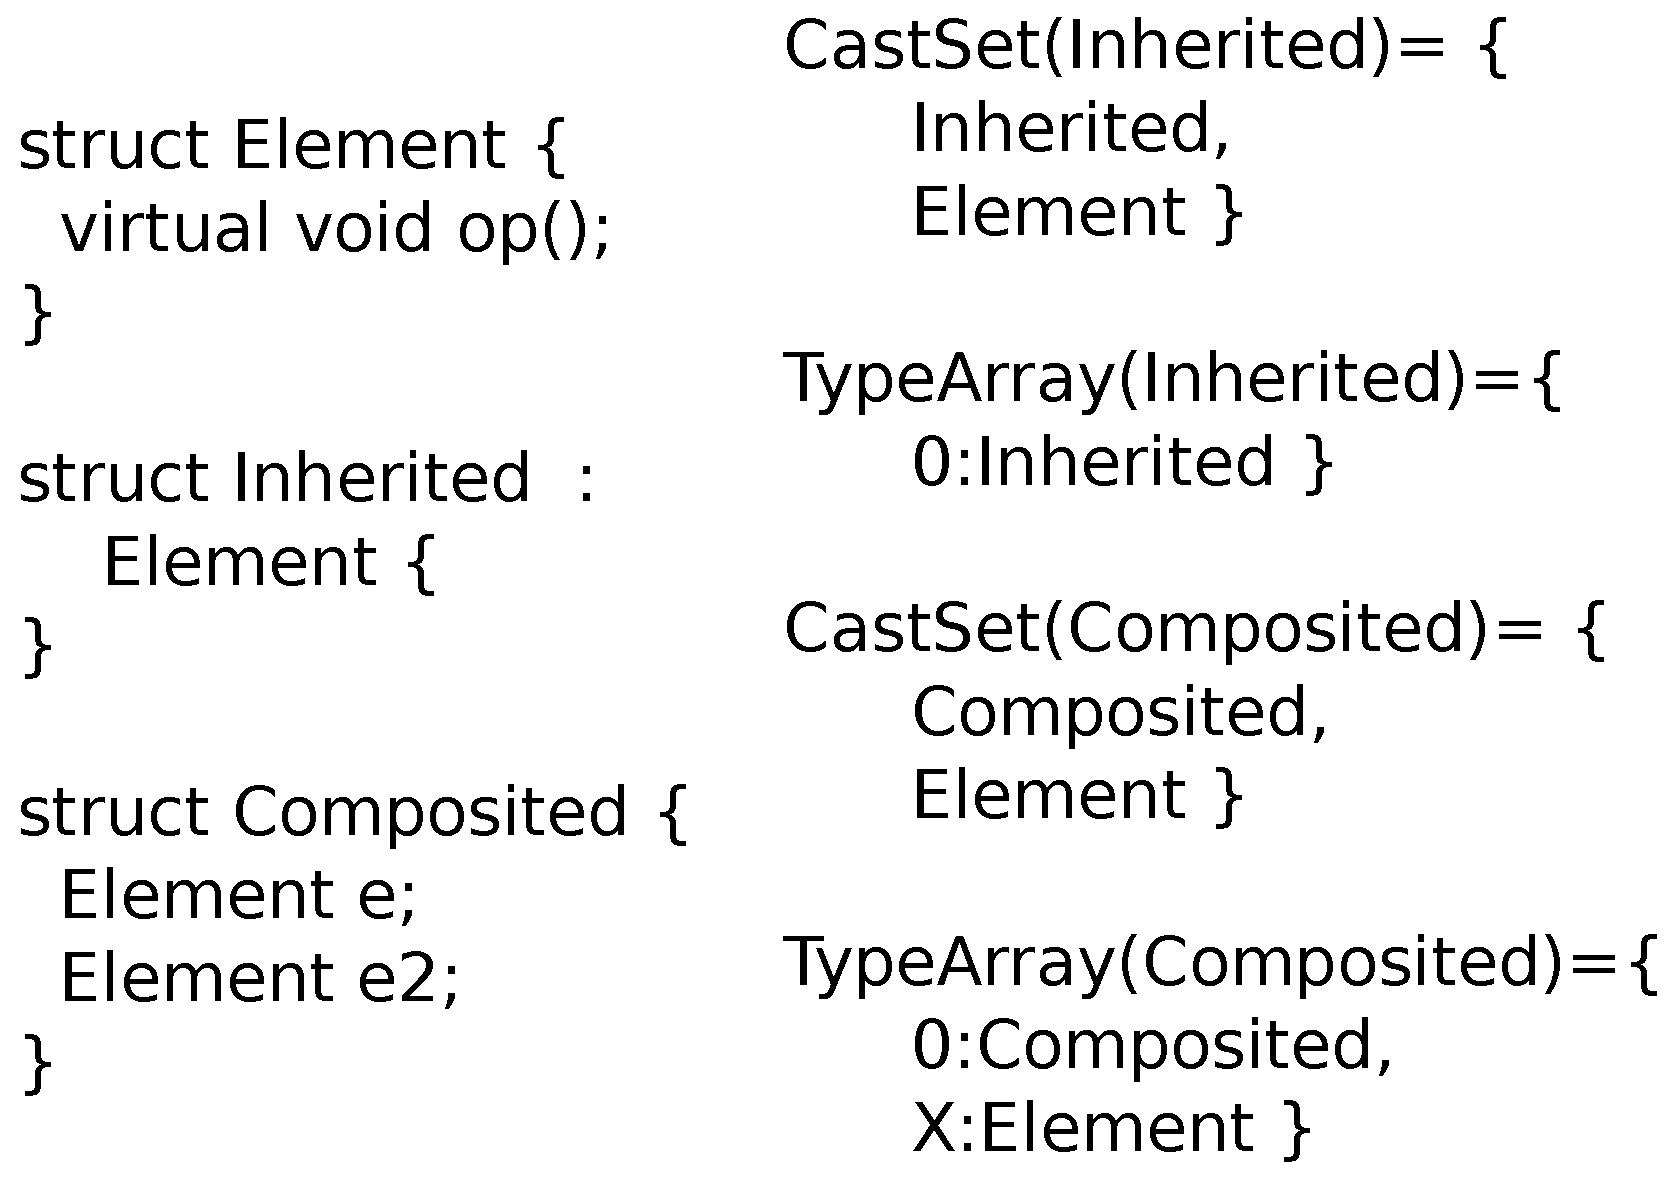
\includegraphics[width=2.8in]{figs/typeexample.eps}
  \caption{
  Example of the interaction between CastSet and TypeArray. For both inheritance and composition,
  the CastSet includes Element as the new type contains a nested Element object at offset 0. The
  TypeArrays include the type itself at offset 0,
  while including other nested types at different offsets, such as the second Element member in the case of the
  Composited class.
  }
  \label{fig:typeexample}
  \vspace{-1em}
\end{figure}

CastSets and TypeArrays are constructed at compile time and stored in global memory, with
the latter pointing to the appropriate CastSets. Type confusion detection requires that
the instrumentation identifies the base pointer of the object as well as the NestedTypeArray corresponding
to the object. This allows to system to retrieve the appropriate CastSet and to identify if the cast target
is within the allowed set or not. This information can be tracked with a simple 8 byte metadata scheme.
The first metadata corresponding to the object includes a pointer to the NestedTypeArray itself, while subsequent
metadata elements store the relative offset (negative) required to reach the base pointer of the object.
Together with the alignment information retrieved as part of the metadata retrieval process, this gives the
instrumentation all the information it needs to perform type confusion detection. Storing different types of
information in the metadata field adds additional complexity (branch for negative values), but it allows
for smaller metadata sizes and thus allocation-time overhead. For this application the 
metadata retrieval frequency is significantly reduced (only required for static down-casts),
thus we expect that this design is preferable to ensure minimal overhead.

\subsection{Dangling Pointer Detection}

Use-after-free vulnerabilities represent the most prominent attack vectors in today's browser landscape~\cite{lee2015preventing}.
While a lot of effort is invested to detect these vulnerabilities via static analysis and software testing,
they typically manifest in highly specialized contexts, making them hard to detect and to fix preemptively.
As such, a couple of systems have been suggested recently to mitigate the underlying reason for the vulnerabilities,
dangling pointers~\cite{lee2015preventing,younan2015freesentry}. These systems rely on tracking heap allocations and
their connectivity at run time. When an object is freed, the systems identify whether there are any pointers
still pointing into the object being released. These pointers are then set to a benign value of NULL to mitigate
potential memory dereferences using them.

Systems for tracking dangling pointers share an underlying design based on three core
data structures. The first is the object map, which identifies heap objects based on any pointer
into the object itself (at any offset). This is equivalent to object metadata tracking.
DangNull~\cite{lee2015preventing} uses red-black trees to track heap allocations, but as discussed
in section~\ref{sec:introduction}, this scheme is susceptible to heavy and unpredictable overhead.
FreeSentry~\cite{younan2015freesentry} uses a label based system, which is equivalent to the fixed
compression ratio metadata shadowing. This scheme offers
fast fixed-time metadata retrieval, but incurs significant allocation-time and memory overhead. In contrast,
\projectname{} combines low allocation- and  lookup overhead with efficient memory usage.

The second data structure is a pointer map, which maps locations storing pointers with information about the
pointer itself. This is essentially location-specific metadata, thus a hash table is the most appropriate
data structure (as no range lookups are required) and both systems use it. The last data structure is the collection
of pointer to object mappings. This structure is used to accumulate information about all incoming/outgoing pointer
for a particular object.  Outgoing pointers are best tracked using a red-black tree as performed in DangNull to
allow efficient retrieval of the outgoing pointer residing at a particular offset in the object. FreeSentry on the
other hand tracks only incoming pointers which can be stored in a simple linked list instead. The disadvantage of
tracking only incoming pointers, is the difficulty of inferring if the source object of the incoming pointer is
still live in memory or not.

We propose a new dangling pointer tracking scheme inspired by FreeSentry, but using \projectname{} to track
object information. The proposed scheme tracks for each heap object the head of the
incoming pointer list as well as a unique identifier to help with object liveness. For each incoming pointer
we track the identifier of the source object, its base address, the address in memory where the pointer is stored
and the pointer value itself.
A hash table is used to map memory
locations with pointers stored within. Each pointer is represented by a link to the appropriate incoming pointer
element described previously. When a pointer is stored in memory, the old incoming pointer is destroyed and a new
one is created and prepended to the list of the target object. Then a link towards this element is stored in the appropriate
hash table location. When an object is freed, the system looks up the incoming pointer list checking if any of the entries
are still valid. An entry is valid if the specified source object still resides at the specified base pointer (based on the
unique identifier) and if the pointer location still contains the specified pointer value. For all valid entries the value stored
in the pointer location is reset to NULL to ensure no use-after-free vulnerabilities can exist. Figure~\ref{fig:metasentry}
showcases the data-structures described above.

\begin{figure}[t]
\center
  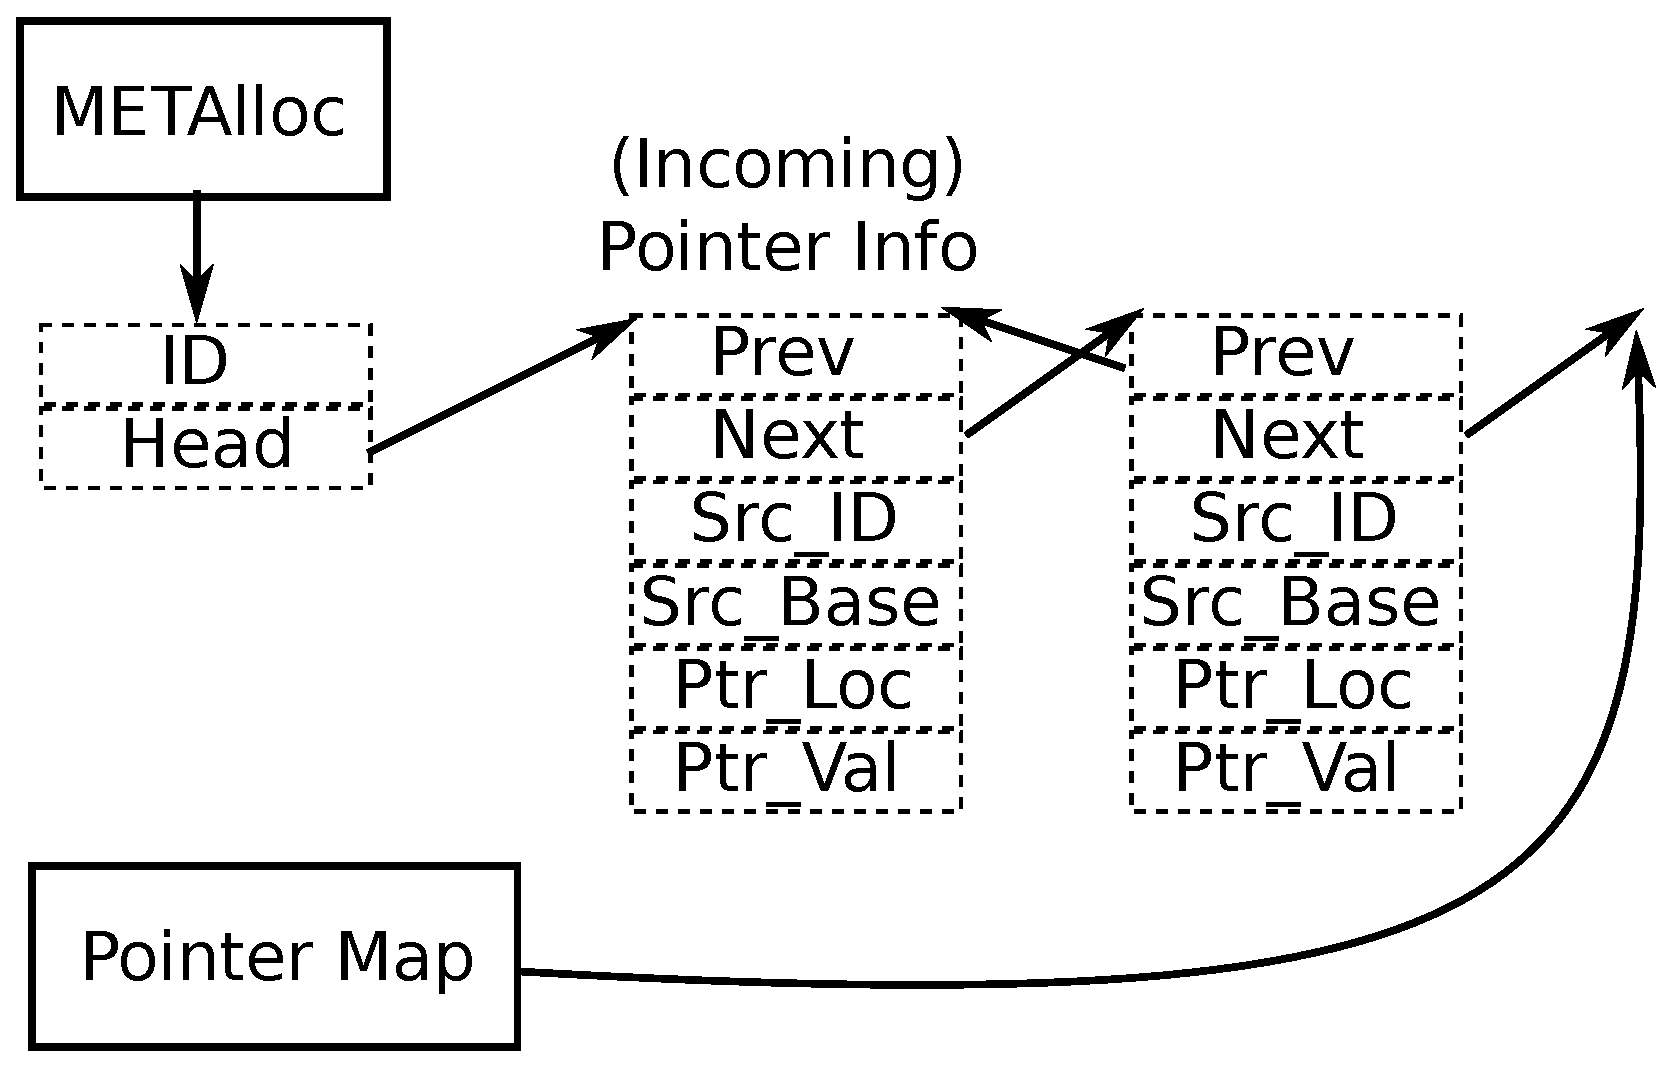
\includegraphics[width=2.8in]{figs/metasentry.eps}
  \caption{
  Data-structures used to implement dangling pointer detection using \projectname{}.
  \projectname{} allows the retreival of a unique object ID as well as a pointer to the head
  of a doubly linked list including information about incoming pointer information. The Pointer Map
  is used to retrieve the pointer infromation corresponding to a pointer stored in a given location.
  For each pointer we store information about the object containing it (ID and base address) as well
  as the location storing the pointer and the pointer value itself to allow nullification.
  }
  \label{fig:metasentry}
  \vspace{-1em}
\end{figure}

\section{Evaluation}
\label{sec:evaluation}

To measure the performance impact of metadata tracking,
we instrumented all the SPECint2006~\cite{henning2006spec} applications to observe the
overhead it introduces. As a baseline, we compiled the applications with
SafeStack enabled since it is advertised as a viable replacement for stack
canaries, even showing lower overhead on some benchmarks~\cite{kuznetsov2014cpi}.
We also use tcmalloc as the heap allocator for our baseline, as it can have
very different run-time performance compared to the system allocator. This decision
is also motivated by the fact that we observed a 5\% improvement of execution
times when using tcmalloc on SPECint2006 (geometric mean). This improvement
increases to 20\% when considering only the C++ benchmarks. The machine used for these
experiments has a Xeon 5620 CPU running Ubuntu 12.04 64-bits.
\looseness=-1

Figure~\ref{fig:spec} shows the overhead introduced with the different configurations
of \projectname{}. We evaluated creating and initializing both 1 and 8-bytes of metadata
for all objects. These setups correspond to different instrumentation types,
like write integrity tracking or type hashes.
The overhead numbers are very low, with the maximum being around 15\% for perlbench and
the geometric mean being $<2$\% for both setups (1.2\% for one byte and 1.5\% for eight bytes). The results also show that metadata size has a
limited impact on the overall performance, showing that the variable compression ratio can help
deal with applications requiring complex metadata. While the measured overhead only includes
the metadata creation and initialization, not the instrumentation itself,
the latter can be tuned with careful design and is the topic
of future work using \projectname{}. To compare \projectname{} against existing metadata tracking
systems, we also implemented and evaluated the metadata shadowing scheme proposed by 
Akritidis et al.~\cite{akritidis2008preventing}. This approach shadows every group of 8
data bytes with a single metadata byte residing within an array allocated at a fixed location.
Even this simple shadowing scheme results in a significantly larger overhead as shown on Figure~\ref{fig:spec}.
The overhead for perlbench explodes to 70\% (going out of bounds in the figure) and the geometric mean across
all benchmarks increases to more than 8\%.

\begin{figure}[t]
\center
  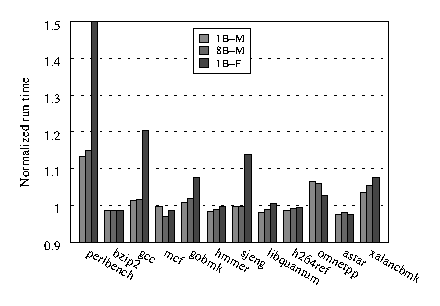
\includegraphics[width=2.8in]{plots/bargraph_runtime_spec.eps}
  \caption{
  SPECint2006 overhead with different configurations of \projectname{}. 1(8)B-M represents the configuration with
  1(8)-byte metadata entries. 1B-F represents the fixed compression ratio metadata shadowing from WIT~\cite{akritidis2008preventing}.
  }
  \label{fig:spec}
  \vspace{-1em}
\end{figure}

\section{Related work}
\label{sec:related}

Besides the different memory shadowing~\cite{akritidis2008preventing,akritidis2009baggy,younan2015freesentry}
and tree-based approaches~\cite{haller2013mempick,lee2015preventing} already discussed within this paper (in Sections~\ref{sec:introduction}
 and~\ref{sec:applications}) there is one system aiming
to solve the metadata tracking problem in a similar manner using a variable compression ratio. The
custom memory allocator implemented within the Sanitizer library of LLVM offers a metadata retrieval system,
which shares characteristics with \projectname{}. The system has been used within CaVer~\cite{lee2015type}
to track type information for heap objects, but is not described in other contexts.

This memory allocator reserves a specific part of the address-space
,as a Region, for each size category defined within the system. Regions are then split into slots of equal
size, with each slot containing a single object. This allows the allocator to associate each slot/object
with a singular piece of metadata, accessed by identifying the slot index corresponding to any pointer.
The Region is also easily identified from the pointer, since the organization of the address-space into
Regions happens at compile-time. This systems shares similarities with \projectname{}, with the primary difference being
the granularity of the memory blobs associated to a certain allocation size. \projectname{} only requires
memory pages to be uniform, which is already assured by the general purpose allocator \emph{tcmalloc}. This custom allocator
on the other hand restricts allocations within a certain Region, whose addresses are predefined at compile-time.
The result is a significant reduction of the potential for address-space randomization, with the address bits
of each Region being predictable by the attackers. Furthermore, the current implementation
also enforces a highly predictable allocation pattern within the Region itself with no ability to release
memory back to the system. The effort to add these highly desirable features to the current design is
unclear at this point. These concerns are of course irrelevant when using the allocator within the desired
context of software testing, but they are key characteristics for a general purpose production allocator.

While the design works efficiently for heap objects, Lee et al.~\cite{lee2015type} argue
that it is not directly applicable to stack and global memory. Their solution to the problem involves
integrating a tree-based metadata tracking for these memory types.
As far as we are aware, \projectname{} is the first design to combine uniformity across memory types with all the advantages
brought forward by variable compression ratio metadata tracking.

\vspace{2em}
\section{Conclusion}
\label{sec:conclusion}

In this paper, we presented \projectname{}, a new memory metadata management scheme
for software security hardening solutions.
Our design is both comprehensive---given that it can handle whole-memory object metadata
in a uniform and transparent way---and efficient---given that it yields a run-time performance
overhead of just 1.2\% in practice.
We believe \projectname{} can bring many instrumentation
solutions within reach for adoption in practice,
allowing, for example, many vulnerability mitigation techniques
to improve software security in an efficient and backward compatible fashion.

\begin{comment}
% Omited in the submitted version
\textbf{Acknowledgment}
This work is supported by the European Research Council through project
ERC-2010-StG 259108-ROSETTA, by the Microsoft Research PhD Scholarship
Programme through the project MRL 2011-049.9, by the Netherlands Organisation
for Scientific Research through grant NWO 639.023.309 VICI ``Dowsing'', and by
the European Commission through the project SHARCS under Grant Agreement No.
644571.
\end{comment}


\bibliographystyle{abbrv}
\bibliography{refs}

\end{document}
